\subsection{Rectifier}
\newcommand{\pwidth}{.95\textwidth}

The simulated output from the half-wave rectifier circuit is shown in
Figure~\ref{fig:halfwavePlotV}.  As is shown, the maximum input voltage
is~\SI{17.401}{\volt} (zero-to-peak), implying an RMS voltage
of~\SI{12.3}{\volt} --- just one tenth of a volt higher than the designed value.
%
\begin{figure}[H]
	\centering
	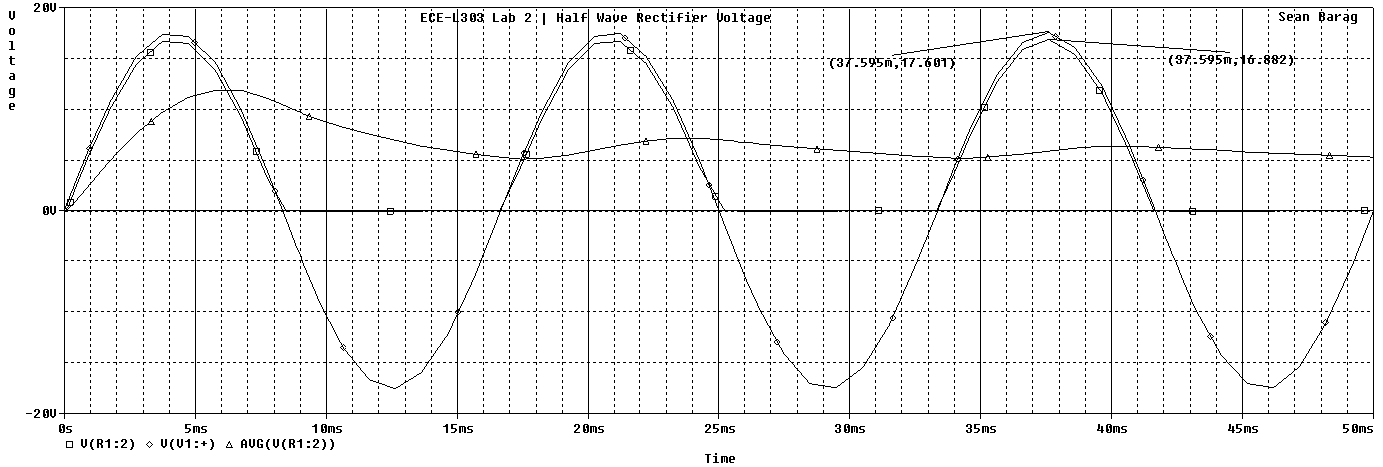
\includegraphics[width=\pwidth]{img/plot/halfwavePlot.PNG}
	\parbox{\pwidth}{
	\caption[PSpice Plot --- Half-wave Rectifier (Voltage)]{PSpice simulated input and }
	\label{fig:halfwavePlotV}}
\end{figure}
%
Similarly, the output had a peak value of~\SI{16.648}{\volt} (zero-to-peak).
After dividing by~$\pi$, the average voltage was found to be~\SI{5.29}{\volt}
--- roughly~\SI{0.3}{\volt} lower than it should be.  The average value of the
output is also plotted on these axes.  As is expected, its value
approaches~\SI{5.29}{\volt} as more input cycles pass.  The decreased average
value is caused by the~\SI{0.7}{\volt} potential drop across the diode required
to turn it on, which is evident in the difference between the peak input and
output values.

An evaluation of power dissipation was also conducted, to ensure that certain
parts would be safe to use.  A plot of power dissipation over time is shown in
Figure~\ref{fig:halfwavePlotW}.
%
\begin{figure}[H]
	\centering
	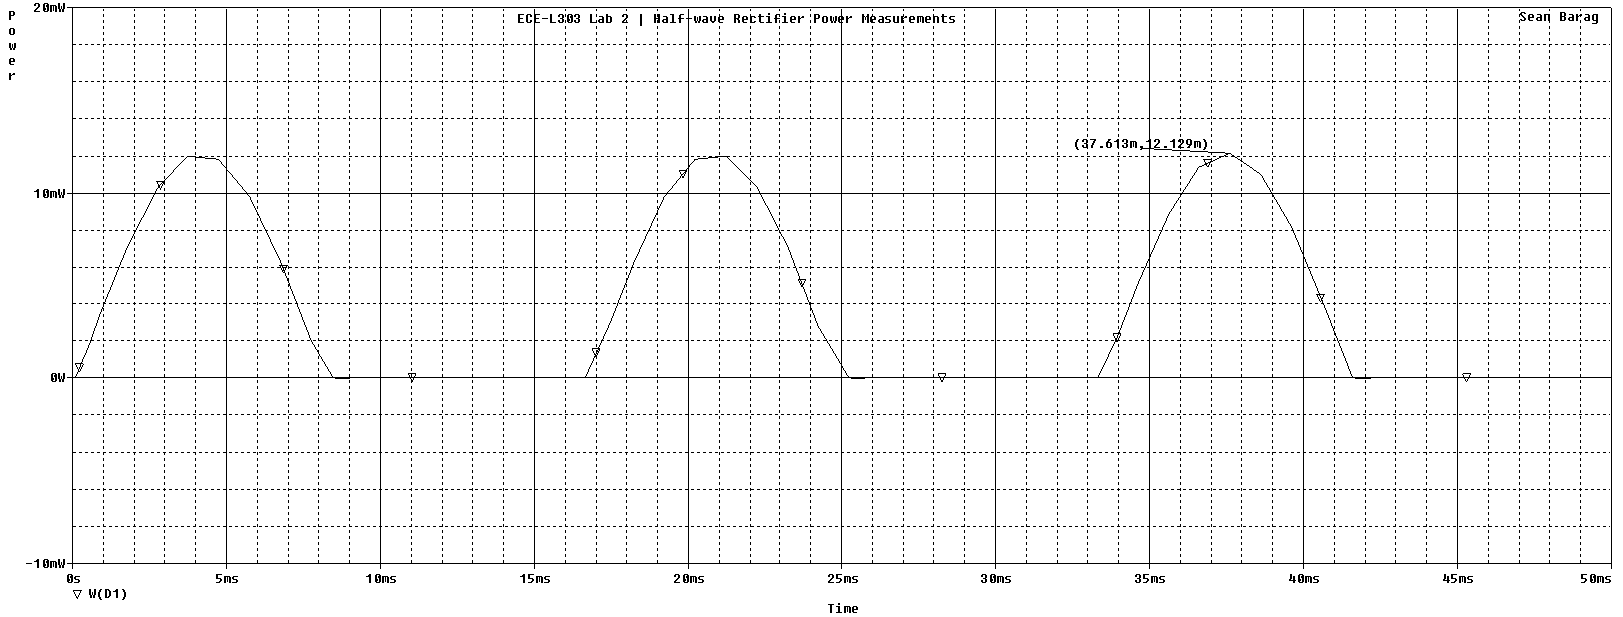
\includegraphics[width=\pwidth]{img/plot/halfwavePowerPlot.PNG}
	\parbox{\pwidth}{
	\caption{}
	\label{fig:halfwavePlotW}}
\end{figure}
%
The maximum power dissipated by the diode is shown as~\SI{12.129}{\milli\watt}.
Any diode with a maximum power dissipation of even one-eighth of a Watt will be
more than sufficient for this circuit.

\subsection{Voltage Regulator}
\begin{figure}[H]
	\centering
	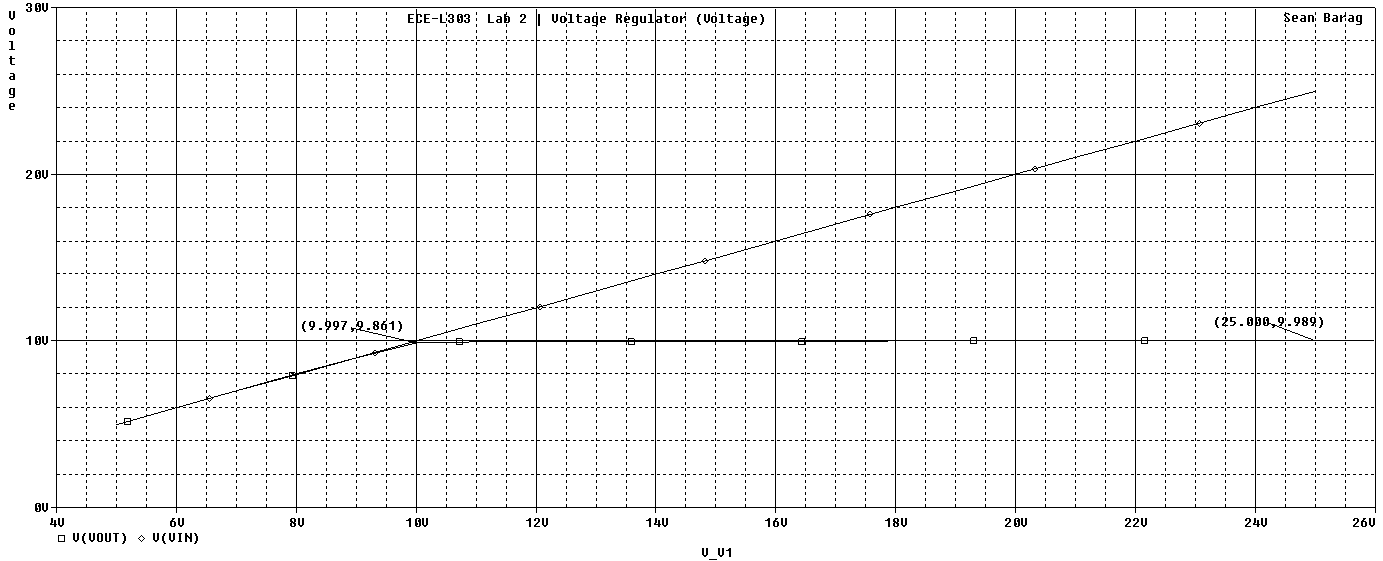
\includegraphics[width=\pwidth]{img/plot/zenerPlot.PNG}
	\parbox{\pwidth}{
	\caption{}
	\label{fig:zenerPlotV}}
\end{figure}

\begin{figure}[H]
	\centering
	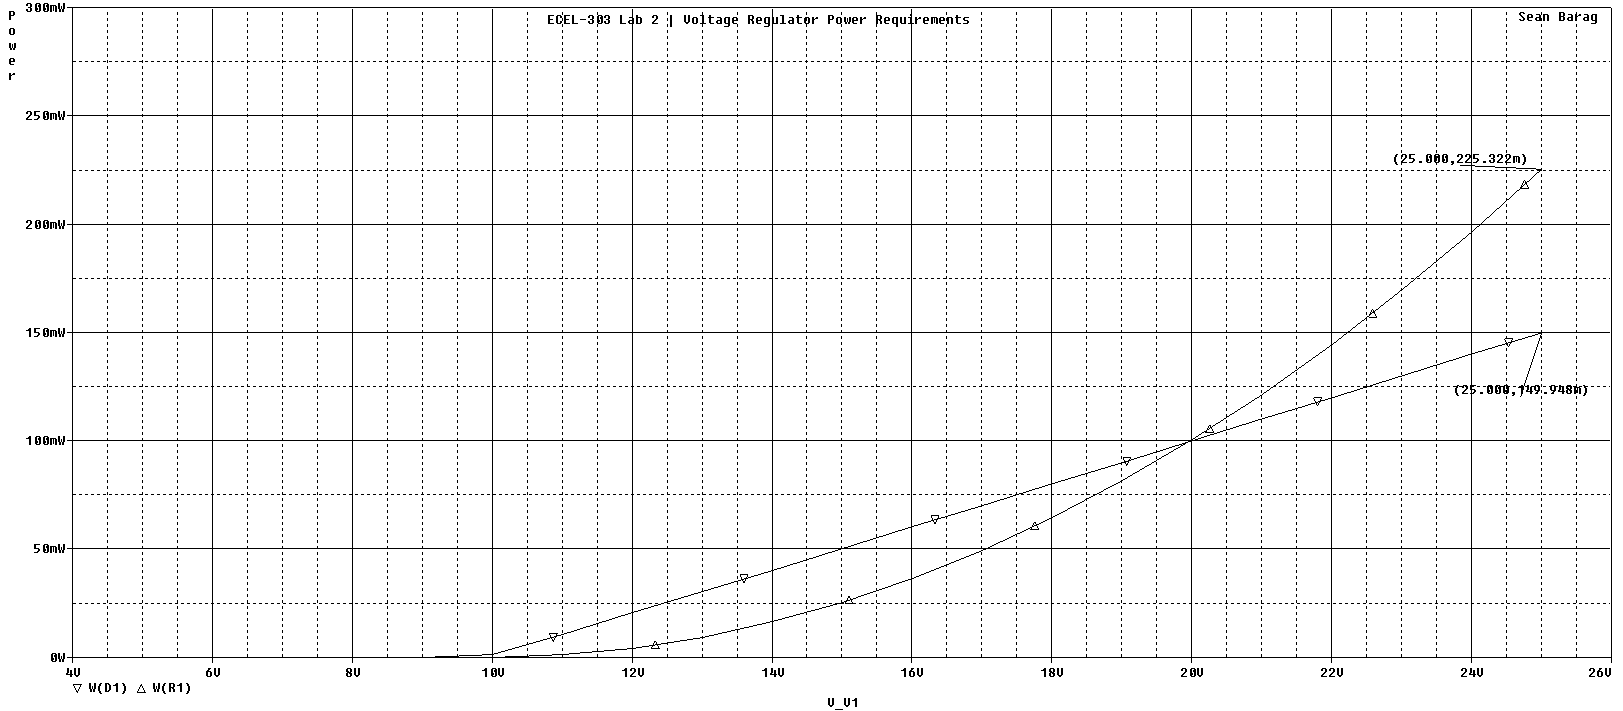
\includegraphics[width=\pwidth]{img/plot/zenerPowerPlot.PNG}
	\parbox{\pwidth}{
	\caption{}
	\label{fig:zenerPlotW}}
\end{figure}

\subsection{Constant Current Source}
\begin{figure}[H]
	\centering
	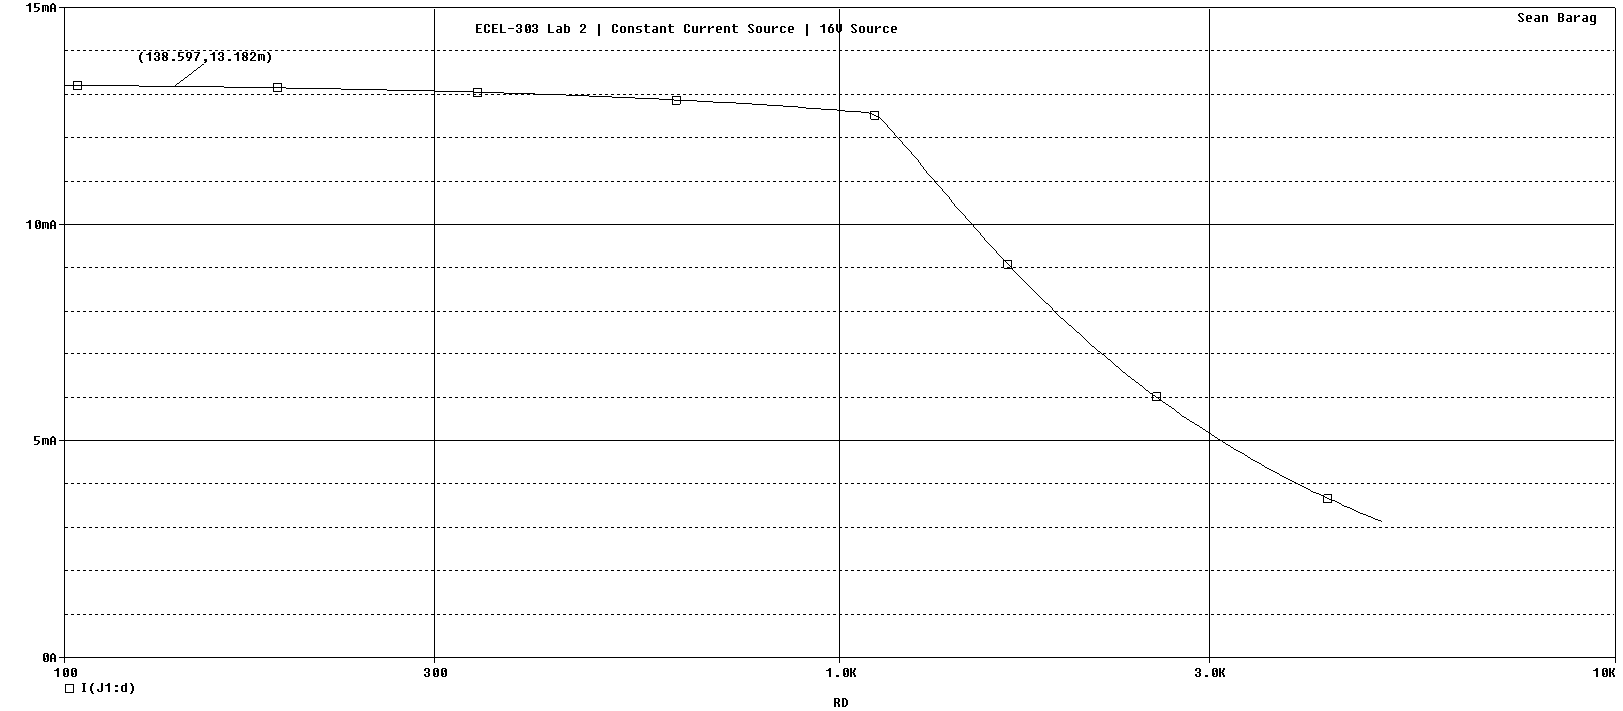
\includegraphics[width=\pwidth]{img/plot/constantCurrent16Plot.PNG}
	\parbox{\pwidth}{
	\caption{}
	\label{fig:ccPlot16}}
\end{figure}

\begin{figure}[H]
	\centering
	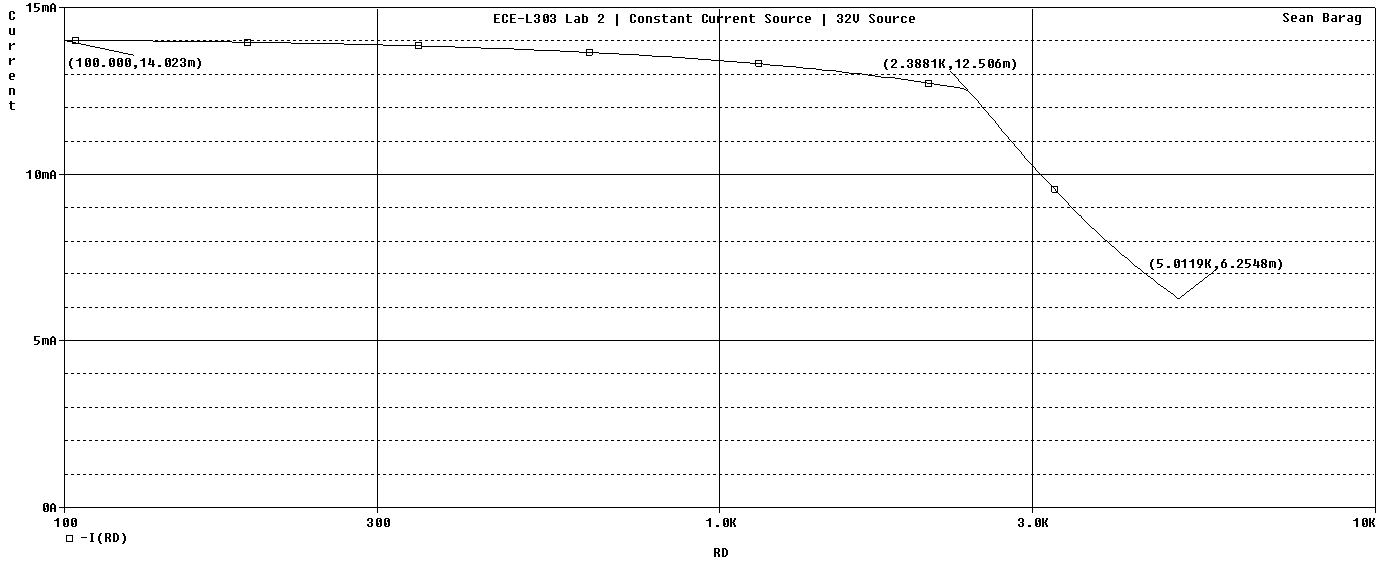
\includegraphics[width=\pwidth]{img/plot/constantCurrent32Plot.PNG}
	\parbox{\pwidth}{
	\caption{}
	\label{fig:ccPlot32}}
\end{figure}

\subsection{High Input Resistance Buffer Amplifier}
\begin{figure}[H]
	\centering
	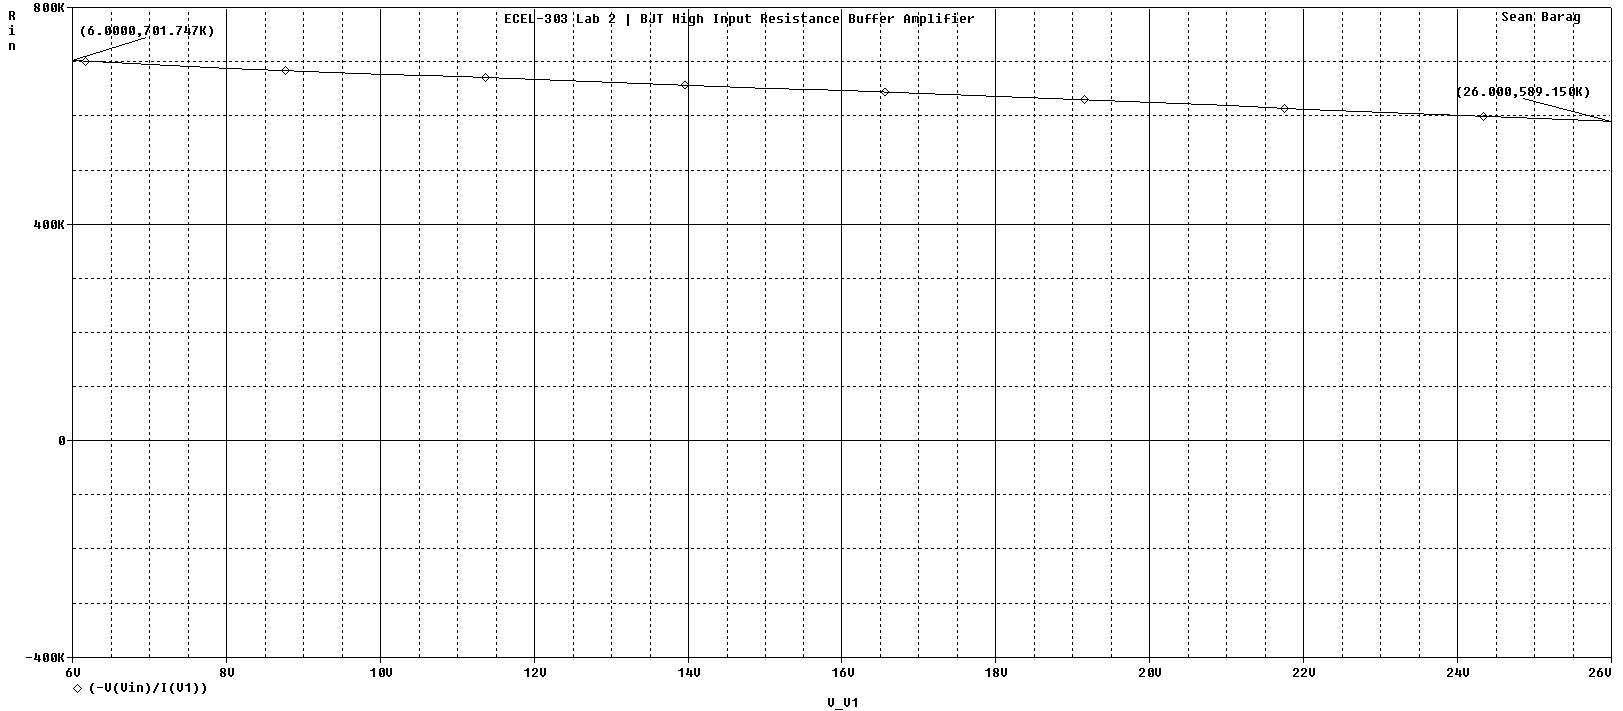
\includegraphics[width=\pwidth]{img/plot/bjtPlotR.PNG}
	\parbox{\pwidth}{
	\caption{}
	\label{fig:bjtPlotR}}
\end{figure}

\begin{figure}[H]
	\centering
	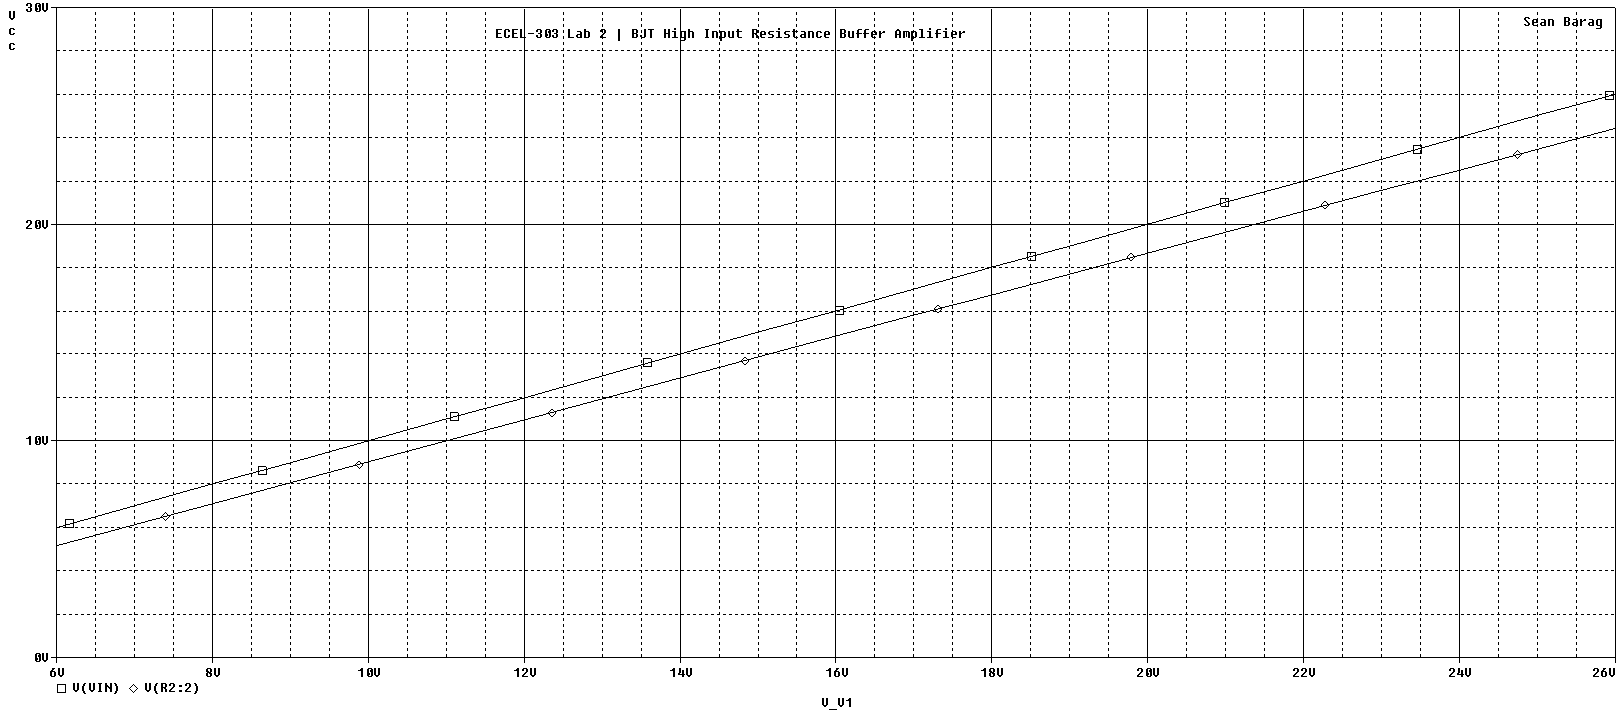
\includegraphics[width=\pwidth]{img/plot/bjtPlotV.PNG}
	\parbox{\pwidth}{
	\caption{}
	\label{fig:bjtPlotV}}
\end{figure}
